\documentclass[letterpaper,twocolumn,10pt]{article}
\usepackage{usenix2019_v3}

% to be able to draw some self-contained figs
\usepackage{tikz}
\usetikzlibrary{positioning,calc,decorations}
\usepackage{amsmath}

% inlined bib file
\usepackage{filecontents}

%-------------------------------------------------------------------------------
\begin{filecontents}{\jobname.bib}
%-------------------------------------------------------------------------------
@Book{arpachiDusseau18:osbook,
  author =       {Arpaci-Dusseau, Remzi H. and Arpaci-Dusseau Andrea C.},
  title =        {Operating Systems: Three Easy Pieces},
  publisher =    {Arpaci-Dusseau Books, LLC},
  year =         2015,
  edition =      {1.00},
  note =         {\url{http://pages.cs.wisc.edu/~remzi/OSTEP/}}
}
@InProceedings{waldspurger02,
  author =       {Waldspurger, Carl A.},
  title =        {Memory resource management in {VMware ESX} server},
  booktitle =    {USENIX Symposium on Operating System Design and
                  Implementation (OSDI)},
  year =         2002,
  pages =        {181--194},
  note =         {\url{https://www.usenix.org/legacy/event/osdi02/tech/waldspurger/waldspurger.pdf}}}
\end{filecontents}

%-------------------------------------------------------------------------------
\begin{document}
%-------------------------------------------------------------------------------

%don't want date printed
\date{}

% make title bold and 14 pt font (Latex default is non-bold, 16 pt)
\title{\Large \bf Secure IVSHMEM Protocol}

%for single author (just remove % characters)
\author{
{\rm Your N.\ Here}\\
Your Institution
\and
{\rm Second Name}\\
Second Institution
% copy the following lines to add more authors
% \and
% {\rm Name}\\
%Name Institution
} % end author

\maketitle




%----------Figure: Channel Separation-----------------
\begin{figure*}[ht]
\begin{center}
  \includegraphics[width=\textwidth]{./figures/channel_separation.png}
\end{center}
\caption{\label{fig:channel_separation} channel separation figure 
  caption's text. }
\end{figure*}
%% %---------------------------

%-------------------------------------------------------------------------------
\begin{abstract}
%-------------------------------------------------------------------------------
Your abstract text goes here. Just a few facts. Whet our appetites.
Not more than 200 words, if possible, and preferably closer to 150.
\end{abstract}


%-------------------------------------------------------------------------------
\section{Introduction}
%-------------------------------------------------------------------------------

The automotive industry is rapidly evolving, driven by advances in semiconductor technology that have shifted system architectures from traditional microcontrollers (MCUs) to powerful Systems-on-Chip (SoCs). This evolution not only enhances computational capabilities but also paves the way for Software-Defined Vehicles (SDVs), where flexibility, scalability, and rapid updates are paramount. In SDVs, virtualization technology plays a crucial role by enabling the coexistence of multiple virtual machines (VMs) on a single hardware platform, ensuring isolated yet efficient execution of diverse applications. For example, modern cockpit domain controllers often deploy separate VMs for real-time operations (RTOS) and infotainment systems, which is essential for balancing performance and safety.

Inter-VM communication in these environments is critical. Traditional approaches, such as TCP/UDP over a network stack or even UART-based messaging, often fall short in terms of speed and resource efficiency. Alternative solutions like VirtIO offer a para-virtualized communication mechanism through ring buffers (VirtQueues), but they do not fully leverage the benefits of shared physical memory. IVSHMEM (Inter-VM Shared Memory) addresses these limitations by mapping each VM's virtualized PCI device to a common physical memory region, allowing rapid data exchange through shared memory. Despite its performance advantages, this method introduces significant security challenges; multiple VMs accessing the same memory space creates vulnerabilities where a compromised or malicious VM could potentially access or modify data belonging to another VM.

This concern is particularly acute in scenarios where critical systems interact with less secure environments. For instance, when an RTOS communicates with an Android-based infotainment VM, there is a tangible risk that a malicious application within Android might tamper with the shared memory region. Such tampering could result in attacks ranging from man-in-the-middle to eavesdropping, ultimately compromising system stability and safety.

In response to these challenges, we propose a secure protocol designed specifically for IVSHMEM communication in automotive systems. Our approach introduces robust security measures on top of the IVSHMEM framework, ensuring data integrity and access control even in an environment with inherent vulnerabilities. While our protocol does introduce some performance overhead, we have implemented novel techniques to mitigate this impact, ensuring that the overhead remains minimal relative to the performance gains achieved by shared memory communication.

In this paper, we provide a detailed analysis of the security threats associated with IVSHMEM, explore the limitations of existing inter-VM communication methods, and describe our protocol's architecture and mitigation strategies. Through comprehensive evaluation, we demonstrate that our secure protocol successfully balances the need for robust security with the high-performance requirements of modern automotive systems and SDVs.

\section{Background}

We explore the evolution of shared memory IPC—from its origins in minimizing data copying in single OS environments to its advanced application in inter-VM communication—and examine the challenges of establishing secure channels over inherently insecure mediums.

\subsection{Shared Memory Inter-Process Communication (IPC)}

Shared memory IPC is a communication mechanism that allows multiple processes running on the same operating system to access a common memory region. This method was originally introduced to avoid redundant data copies between processes, thereby enhancing performance. The concept has been extended to inter-VM communication, where co-located virtual machines (VMs) on the same host exchange data via a shared memory channel. Instead of routing data through the host operating system or hypervisor—an approach that incurs additional overhead—the sender VM writes data directly into a shared memory region and then notifies the receiver VM via an interrupt. This streamlined process significantly accelerates communication between VMs.


OpenMPI - Job Isolation?
Boost Interprocess?

\subsection{IVSHMEM: Mechanism and Architecture}


IVSHMEM (Inter-VM Shared Memory) is a specialized implementation of shared memory IPC designed for virtualized environments. It emulates a virtual PCI device to expose the shared memory's base address and size to guest VMs. The design leverages the standardized PCI configuration to facilitate memory mapping and efficient communication. Specifically, IVSHMEM utilizes:

- **BAR0 (Base Address Register 0):** This region (256 bytes of MMIO) holds the device registers, which control the operation of the virtual device.
- **BAR1:** It contains the MSI-X table and Pending Bit Array (PBA), primarily used by the IVSHMEM doorbell mechanism for signaling interrupts.
- **BAR2:** This is mapped to the shared memory object, providing a direct communication channel between VMs.

The doorbell interrupt mechanism enabled by this configuration allows VMs to notify one another when new data is available, ensuring efficient core utilization and reducing latency in inter-VM communication.

%----------Figure: handshake -----------------
\begin{figure}[ht]
\begin{center}
  \includegraphics[width=0.95\linewidth]{./figures/ivshmem_arch.png}
\end{center}
\caption{\label{fig:ivshmem_arch} IVSHMEM architecture figure 
  caption's text. }
\end{figure}
%% %---------------------------




\subsection{Security Concerns of Shared Memory}
While shared memory IPC within a single operating system benefits from well-established security mechanisms—such as file access controls, sandboxing, and enhanced security modules like SELinux or AppArmor—IVSHMEM presents unique challenges. In a traditional OS environment, the operating system enforces strict access controls over shared memory regions, ensuring that only authorized processes can read or write data. However, when multiple, potentially untrusted VMs share the same memory space, these protections are significantly diminished. A compromised or malicious VM could easily access or tamper with data in the shared region, leading to unauthorized data disclosure, corruption, or even system instability. This risk is compounded by the fact that the emulated PCI device, which exposes the shared memory, does not inherently enforce robust access control policies among the VMs.


\subsection{Secure Communication Over Insecure Channels}

The challenge of ensuring secure communication in IVSHMEM environments is analogous to securing communication over the Internet, where multiple parties exchange information over an inherently insecure channel. In the realm of network communications, protocols such as TLS rely on key exchange mechanisms, mutual authentication, and end-to-end encryption to safeguard data integrity and confidentiality. Similarly, secure multi-party communication techniques—such as Diffie-Hellman key exchange and advanced encryption standards—are employed to establish trust even when the channel is compromised.

In the context of IVSHMEM, the situation is even more complex because multiple services must share the same restricted memory space as a communication channel. This necessitates the design of a secure protocol that not only ensures confidentiality and integrity—akin to TLS or other network security protocols—but also accommodates the shared nature of the memory resource. Our research addresses these challenges by proposing a secure protocol that implements robust cryptographic techniques to protect the data transmitted via IVSHMEM, while also mitigating the performance overhead typically associated with such security measures.



Through this background, we highlight the evolution from traditional shared memory IPC to advanced inter-VM communication methods like IVSHMEM, outline its architectural underpinnings, and discuss the critical security concerns that arise when untrusted VMs share a common memory resource. This sets the stage for our proposed solution, which aims to secure inter-VM communication in automotive systems without compromising on the performance benefits of shared memory mechanisms.




\section{The need for Secure IVSHMEM Protocol}

blah

\subsection{Threat Model}


untrusted VMs
replay attacks
man in the middle attacks
eavesdropping



\subsection{General Purpose of Secure IVSHMEM Protocol}

blah blah blah

\subsection{Performance Optimization}

blah blah blah



\section{Design Proposal (or) Secure IVSHMEM Protocol}

blah blah blah




\subsection{Service-based Channel division}
blah blah blah

\subsection{Granualr Access Control}

blah blah blah


\subsection{Hypervisor Mediated Handshake Protocol}




%----------Figure: handshake -----------------
\begin{figure}[ht]
\begin{center}
  \includegraphics[width=0.95\linewidth]{./figures/ivshmem_handshake.png}
\end{center}
\caption{\label{fig:handshake} handshake figure 
  caption's text. }
\end{figure}
%% %---------------------------



blah blah blah


\subsection{Channel-based Data Transfer}

\subsubsection{Dynamic Channel Rebalancing}

blah blah blah

\subsubsection{Lock-free Data Transfer}

blah blah blah

\subsubsection{Bi-directional Ring Buffer}

blah blah blah
Yoo Jung Cuttie


\section{Implementation}

blah blah blah


\section{Performance Mitigation}

blah blah blah

\section{Related Work}

blah blah blah

\section{Conclusion}

blah blah blah

\section*{Acknowledgments}

Thanks to all the people who helped me.





%-------------------------------------------------------------------------------
\section{Footnotes, Verbatim, and Citations}
%-------------------------------------------------------------------------------

Footnotes should be places after punctuation characters, without any
spaces between said characters and footnotes, like so.%
\footnote{Remember that USENIX format stopped using endnotes and is
  now using regular footnotes.} And some embedded literal code may
look as follows.

\begin{verbatim}
int main(int argc, char *argv[]) 
{
    return 0;
}
\end{verbatim}

Now we're going to cite somebody. Watch for the cite tag. Here it
comes. Arpachi-Dusseau and Arpachi-Dusseau co-authored an excellent OS
book, which is also really funny~\cite{arpachiDusseau18:osbook}, and
Waldspurger got into the SIGOPS hall-of-fame due to his seminal paper
about resource management in the ESX hypervisor~\cite{waldspurger02}.

The tilde character (\~{}) in the tex source means a non-breaking
space. This way, your reference will always be attached to the word
that preceded it, instead of going to the next line.

And the 'cite' package sorts your citations by their numerical order
of the corresponding references at the end of the paper, ridding you
from the need to notice that, e.g, ``Waldspurger'' appears after
``Arpachi-Dusseau'' when sorting references
alphabetically~\cite{waldspurger02,arpachiDusseau18:osbook}. 

It'd be nice and thoughtful of you to include a suitable link in each
and every bibtex entry that you use in your submission, to allow
reviewers (and other readers) to easily get to the cited work, as is
done in all entries found in the References section of this document.

Now we're going take a look at Section~\ref{sec:figs}, but not before
observing that refs to sections and citations and such are colored and
clickable in the PDF because of the packages we've included.

%-------------------------------------------------------------------------------
\section{Floating Figures and Lists}
\label{sec:figs}
%-------------------------------------------------------------------------------


%---------------------------
\begin{figure}
\begin{center}
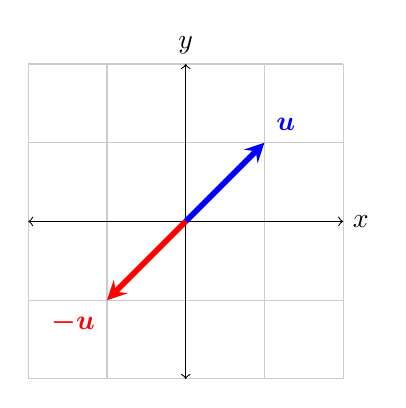
\begin{tikzpicture}
  \draw[thin,gray!40] (-2,-2) grid (2,2);
  \draw[<->] (-2,0)--(2,0) node[right]{$x$};
  \draw[<->] (0,-2)--(0,2) node[above]{$y$};
  \draw[line width=2pt,blue,-stealth](0,0)--(1,1)
        node[anchor=south west]{$\boldsymbol{u}$};
  \draw[line width=2pt,red,-stealth](0,0)--(-1,-1)
        node[anchor=north east]{$\boldsymbol{-u}$};
\end{tikzpicture}
\end{center}
\caption{\label{fig:vectors} Text size inside figure should be as big as
  caption's text. Text size inside figure should be as big as
  caption's text. Text size inside figure should be as big as
  caption's text. Text size inside figure should be as big as
  caption's text. Text size inside figure should be as big as
  caption's text. }
\end{figure}
%% %---------------------------


Here's a typical reference to a floating figure:
Figure~\ref{fig:vectors}. Floats should usually be placed where latex
wants then. Figure\ref{fig:vectors} is centered, and has a caption
that instructs you to make sure that the size of the text within the
figures that you use is as big as (or bigger than) the size of the
text in the caption of the figures. Please do. Really.

In our case, we've explicitly drawn the figure inlined in latex, to
allow this tex file to cleanly compile. But usually, your figures will
reside in some file.pdf, and you'd include them in your document
with, say, \textbackslash{}includegraphics.

Lists are sometimes quite handy. If you want to itemize things, feel
free:

\begin{description}
  
\item[fread] a function that reads from a \texttt{stream} into the
  array \texttt{ptr} at most \texttt{nobj} objects of size
  \texttt{size}, returning returns the number of objects read.

\item[Fred] a person's name, e.g., there once was a dude named Fred
  who separated usenix.sty from this file to allow for easy
  inclusion.
\end{description}

\noindent
The noindent at the start of this paragraph in its tex version makes
it clear that it's a continuation of the preceding paragraph, as
opposed to a new paragraph in its own right.


\subsection{LaTeX-ing Your TeX File}
%-----------------------------------

People often use \texttt{pdflatex} these days for creating pdf-s from
tex files via the shell. And \texttt{bibtex}, of course. Works for us.

%-------------------------------------------------------------------------------
\bibliographystyle{plain}
\bibliography{\jobname}

%%%%%%%%%%%%%%%%%%%%%%%%%%%%%%%%%%%%%%%%%%%%%%%%%%%%%%%%%%%%%%%%%%%%%%%%%%%%%%%%
\end{document}
%%%%%%%%%%%%%%%%%%%%%%%%%%%%%%%%%%%%%%%%%%%%%%%%%%%%%%%%%%%%%%%%%%%%%%%%%%%%%%%%

%%  LocalWords:  endnotes includegraphics fread ptr nobj noindent
%%  LocalWords:  pdflatex acks


